\documentclass[twocolumn,a4paper]{article}
\usepackage[utf8]{inputenc}
\usepackage[T1]{fontenc}
\usepackage{amsmath}
\usepackage{amssymb}
\usepackage{graphicx}

\usepackage[margin=2cm]{geometry}

\author{Josh Pattman}
\title{Evolutionary Learning In Grouped Gene Networks}
\begin{document}
	\maketitle
    \section{Introduction}
    Two of the most important features when describing an organism are its genotype and its phenotype. A genotype encompasses the entire genetic code of an organism, while the phenotype is the physical manifestation of that code. However, the relationship between a genotype and a phenotype is a complex one, as a single locus in the genotype does not hold a one-to-one relationship with a single trait in the phenotype. Instead, the phenotype is the result of the entire genotype interacting with the gene regulation network (GRN) of the organism.

    A GRN is a mechanism by which the various genes in the genotype interact with each other to eventually reach a stable state describing the phenotype. Each node in the GRN represents a locus in the genotype and phenotype, and connections between nodes represent the interactions between genes. The GRN is not fixed throughout generations, but instead evolves alongside the genotypes of the organisms, with each organism having its own unique GRN. However, the rate of evolution of the GRN is significantly slower than that of the genotype, meaning that the GRN may reatin information from previous fitness landscapes, even if that information is not immidiately useful to a given organism at the present time.

    Evolved GRNs have a nubmer of interesting properties. For example, a GRN may recognise genes which frequently covary, and increase the likelihood of those genes being expressed together. A GRN also may take advantage of its ability to retain information from previous fitness landscapes to increase the likelihood of a group of traits from that landscape being expressed in the future. This is particularly useful in nature, as a previously proven trait of a creature may be more helpful in a future environment than a new randomly evolved one. This ability of a GRN to remember previous fitness landscapes is refered to as genetic memory.

    This paper aims to investigate the effects of genetic memory in a variety of scenarios, building upon previous work by Richard A. Watson Et al. CITEME, henceforth referered to as the previous work. In the previous work, a mathematical model for a genotype and GRN was created, and hill climbing was performed to optimise a GRN to commit multiple phenotypes to memory. The trained GRN was then used to produce various combinations of the training phenotypes upon being presented with a random genotypic input.

    The previous work also showed that, using their specific method, the weights of the GRN tended to move towards the weights acheived by hebbian learning on the training data. This result is significant, as it suggests a hill climbing algorithm may in part be equivalent to more traditional 'intelligent' machine learning algorithms.

    \section{Experiment Setup}
    This paper first reimplements the algorithms from the previous work, and then reproduces the results obtained by that paper. For that reason, a genotype of an individual is represented by a vector $G$. This vector can contain any values, but in practice these values stay as small numbers centered around zero.
    
    The GRN is represented by an interaction matrix $B$, which has the same number of rows and columns as there are elements in $G$. The state of the GRN at time $t$ is represented by a vector $P(t)$, which is governed by (\ref{eq:origpa}) and (\ref{eq:origp}).
    \begin{equation} \label{eq:origpa}
        P(1) = G
    \end{equation}
    \begin{equation} \label{eq:origp}
        P(t+1) = P(t) + \tau_1 \sigma (B P(t)) - \tau_2 P(t)
    \end{equation}
    Where $\tau_1$ and $\tau_2$ are the update rate and decay rate of the network respectively, and $\sigma$ is the $tanh$ function. The final phenotype on which the fitness is evaluated is given by $P(t_{final})$, where $t_{final}$ is set to 10 for all tests in this paper.

    The fitness function is a modified version of that used in the previous work and is given by (\ref{eqn:fitness}).
    \begin{equation} \label{eqn:fitness}
        |{sum} (P \odot T)|
    \end{equation}
    In this equation, $P$ is the produced phenotype, $T$ is the target phenotype, and $\odot$ is the element-wise multiplication operator. Using this function, a value of 0 is minimally fit, but the fitness can extend to positive infinity. The reason for taking the absolute is that a perfect negative of the produced phenotype is indistinguishable from the target phenotype for the GRN. In the previous work, the fitness function would penalise a perfect negative, however this paper chooses to reward this.

    The genetic algorithm (GA) used in this paper is a simple point mutation hill climbing model. At any given step, there exist two individuals. One of these represents the previous best individual, and the other is a mutated version of the previous best. At each step, the mutated individual is re-initialised to the previous best, then a random point mutation is applied to both its genotype and GRN. If the mutated individual has a higher fitness than the previous best, it becomes the new previous best. This process is repeated for a set number of iterations, and the final best individual is returned. It is very important that the point mutation size of the GRN is significantly smaller than that of the genotype, otherwise the GRN may overwrite previously learned information. Mutations are either a uniformly or normally distributed random number, which is added to the previous value of the gene.

    \section{Reimplemented Results 1pg}
    \begin{figure}[h]
        \centering
        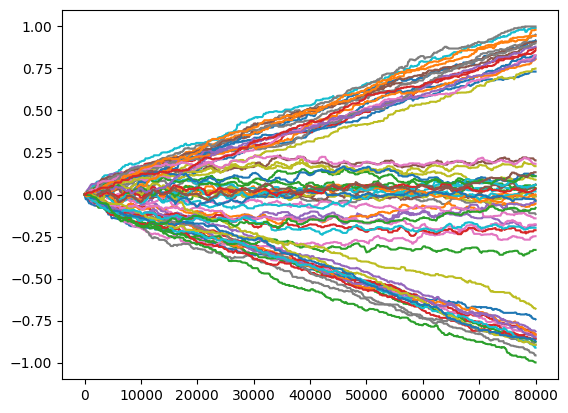
\includegraphics[width=0.48\linewidth]{img/fig2a.png}
        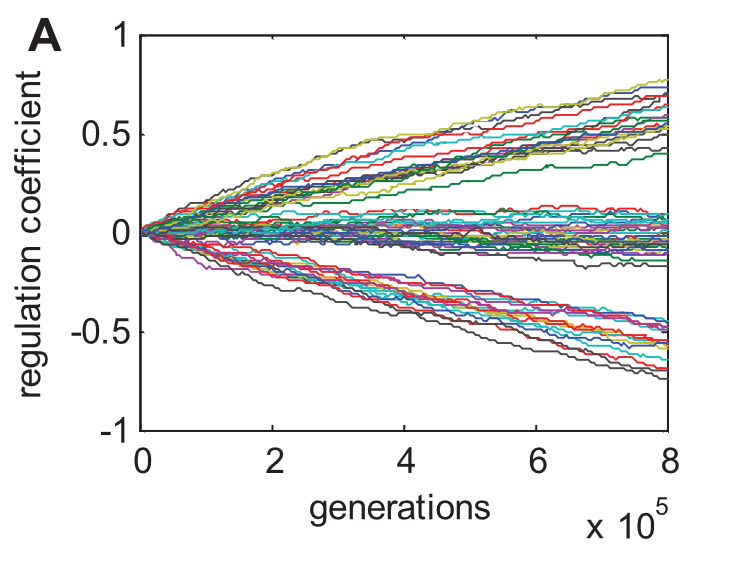
\includegraphics[width=0.48\linewidth]{orig_img/fig2a.png}
        \caption{On the left, the original paper. On the right, the reimplemented results.}
    \end{figure}

    \begin{figure}[h]
        \centering
        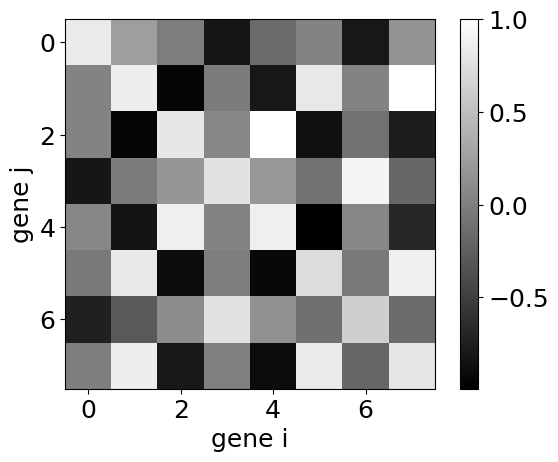
\includegraphics[width=0.48\linewidth]{img/fig2b.png}
        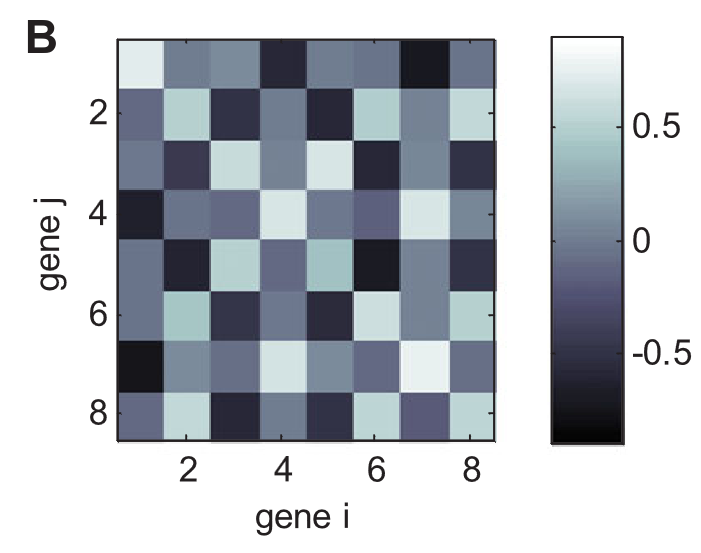
\includegraphics[width=0.48\linewidth]{orig_img/fig2b.png}
        \caption{On the left, the original paper. On the right, the reimplemented results.}
    \end{figure}

    \begin{figure}[h]
        \centering
        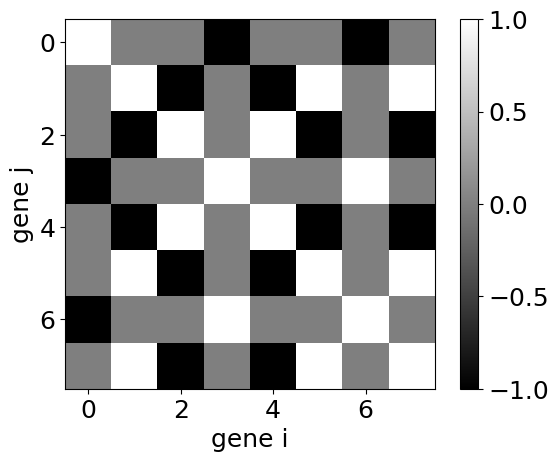
\includegraphics[width=0.48\linewidth]{img/fig2c.png}
        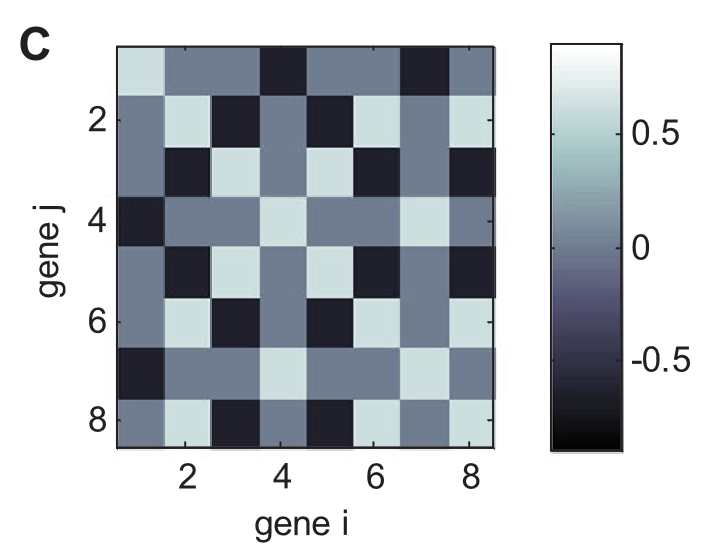
\includegraphics[width=0.48\linewidth]{orig_img/fig2c.png}
        \caption{On the left, the original paper. On the right, the reimplemented results.}
    \end{figure}

    \begin{figure}[h]
        \centering
        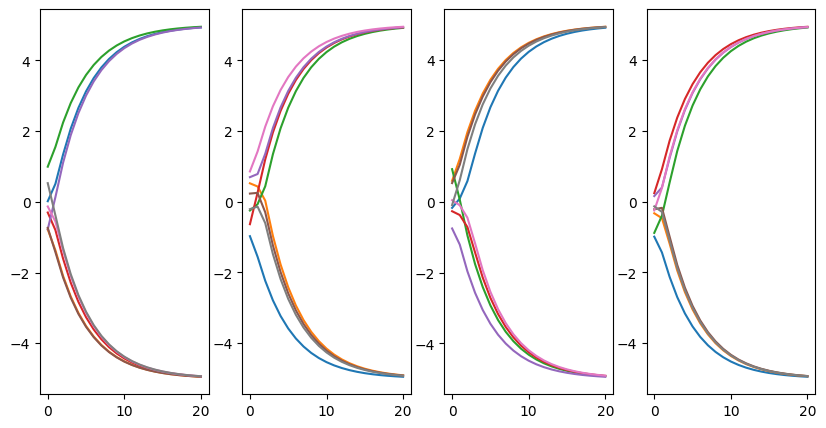
\includegraphics[width=0.9\linewidth]{img/fig2d.png}
        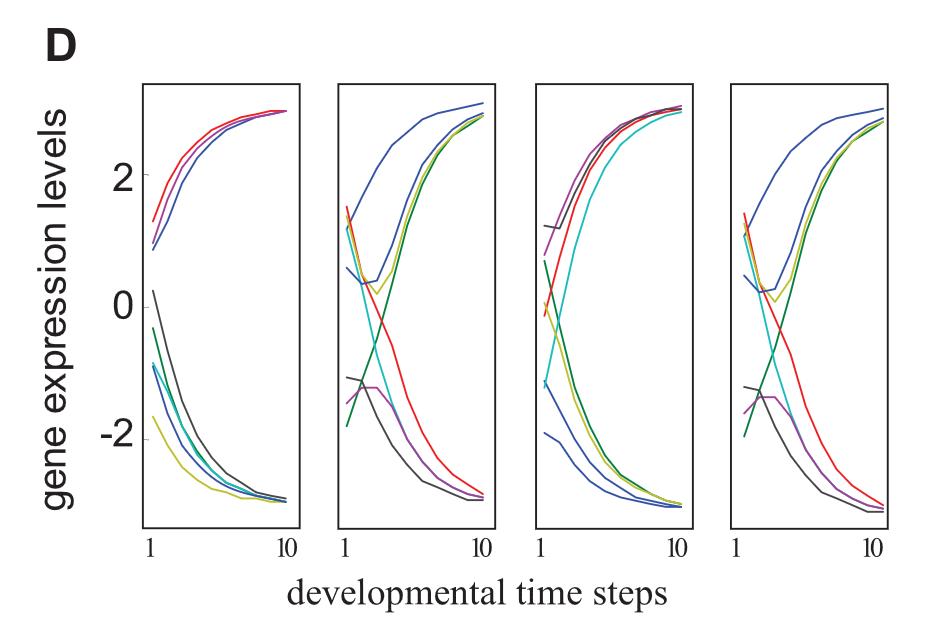
\includegraphics[width=0.9\linewidth]{orig_img/fig2d.png}
        \caption{On the left, the original paper. On the right, the reimplemented results.}
    \end{figure}

    \begin{figure}[h]
        \centering
        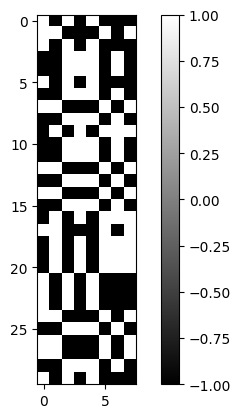
\includegraphics[width=0.45\linewidth]{img/fig2e.png}
        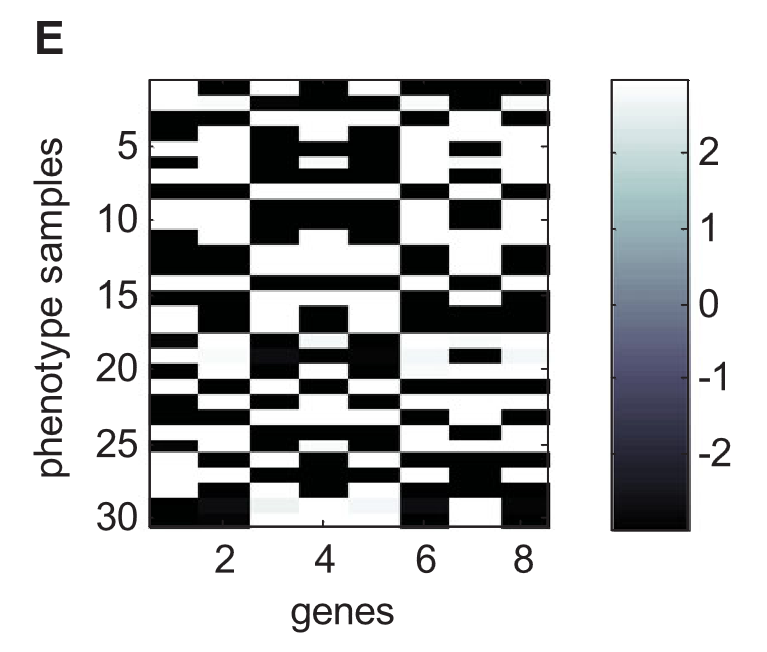
\includegraphics[width=0.45\linewidth]{orig_img/fig2e.png}
        \caption{On the left, the original paper. On the right, the reimplemented results.}
    \end{figure}

    \begin{figure}[h]
        \centering
        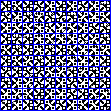
\includegraphics[width=0.45\linewidth]{img/fig4b.png}
        \caption{Bestiary of genotypes reimplemented to the specification of Figure 4 in the original paper.}
    \end{figure}

    \begin{itemize}
        \item 1 Page
        \item The reimplemented figures (side by side with the originals)
        \item Discussion of what the results show/don't show, what worked/didn't work, what you learned
    \end{itemize}
    \section{Extension 1pg}
    The previously described model of a GRN is a significant abstraction of the true complexity of the interactions between genes. To extend this work, this paper proposes a more advanced model of a GRN which takes inspiration from protein production in genes.

    In a biological GRN, the expression level of a gene is affected not directly by the expression levels of other genes, but instead by the levels of protiens produced by those genes. It also may be the case that there are significantly fewer unique protiens available for this purpose than there are genes, meaning that genes with similar functions may have to evolve to use similar proteins for regulation. These features of GRNs are not caputered by using a single regulation matrix to represent the interaction between genes.

    \subsection{Goals and Hypothesis}
    This extension focusses on simulating these intermediate messenger proteins in a simplified manner while maintaining maximum similarity with the previously described method, enabling simple comparisons between the two.

    The hypothesis of this experiment is two-fold:
    \begin{enumerate}
        \item \textbf{The gene regulation network will be able to remember previously expressed phenotipic patterns even with an overall reduction in the number of parameters when compared to a dense network.} This is because in the datasets used for these experiments, and indeed real life, there are patterns that the network should be ableto encode into a single protien. Each pattern may then also affect multiple genes in a similar way. These features leave much room for the network to genralise and group certain features that behave in similar ways together.
        \item \textbf{The gene regulation network may become more robust and better at genralising to new patterns, as it is forced to 'make sense' of the input genotype.} In traditional machine learning, a bottleneck is a point in a model where there are fewer features than there were inputs to the model, forcing the network to learn the patterns in its data rather than memerising it. Hypothetically, this should also apply to a GRN with fewer chemicals than genes, as the GRN will need to extract only the most important information from the inputs in order to best create an accurate output.
    \end{enumerate}

    \subsection{Model}
    To represent this new model of a GRN, the interaction matrix must be replaced by two distinct matricies, one for encoding a state of the GRN into a vector representing the protein production, $B_e$, and one for decoding a protien production vector into the updates to each state, $B_d$. Given a number of available proteins $n_{protein}$ and the genotype size $n_{genotype}$, $B_e$ has dimensions $(n_{protein},n_{genotype})$, and $B_d$ has dimensions $(n_{genotype},n_{protein})$. Given these matricies the phenotype at the next timestep, column vector $P(t+1)$, is given by the equation
    \begin{equation}
        P(t+1) = P(t) + \tau_1 \sigma (B_d (B_e P(t))) - \tau_2 P(t)
    \end{equation}
    Where $\tau_1$ and $\tau_2$ are the update rate and decay rate of the network respectively, and $\sigma$ is the sigmoid function.

    This method has some useful properties aside from furfilling the aim to simulate the intermediate properties:
    \begin{enumerate}
        \item Mapping the previous state to the next state with two matricies may be a faster computation with fewer parameters compared to a single interaction matrix, as long as
        \begin{equation}
            n_{protien} < n_{genotype} \div 2
        \end{equation}
            
        \item As the matricies are multiplied linearly together, it is possible to find the equivalent single interaction matrix by performing the calculation
        \begin{equation}
            B = B_dB_e
        \end{equation}
        Computing the single interaction matrix enables easy comparison to both the original approach, and the weights derived from Hebbs rule, which is useful when evaluating if this model maintains the tendancy to move towards the Hebbian weights.
    \end{enumerate}
    \begin{itemize}
        \item TODO: Support the value of asking that question (using literature)
    \end{itemize}


    \section{Extension Results}
    \begin{itemize}
        \item 1.5 page
    \end{itemize}


    \section{Conclusion}
    \begin{itemize}
        \item one page
        \item What do you conclude from that
        \item significance of the extension results
        \item critique/evaluation
    \end{itemize}


    \section{Appendix}


\end{document}